%%%%%%%%%%%%%%%%%%%%%%%%%%%%%%%%%%%%%%%%%%%%%%%%%%%%%%%%%%%%%%%%%%%%%
\documentclass[letterpaper]{physor2018}
%
%  various packages that you may wish to activate for usage
\usepackage{tabls}
\usepackage{cites}
\usepackage{epsf}
\usepackage{appendix}
\usepackage{ragged2e}
\usepackage[top=1in, bottom=1.in, left=1.in, right=1.in]{geometry}
\usepackage{enumitem}
\setlist[itemize]{leftmargin=*}
\usepackage{caption}
\captionsetup{width=1.0\textwidth,font={bf,normalsize},skip=0.3cm,within=none,justification=centering}
\usepackage{xspace}

%\usepackage[justification=centering]{caption}

\newcommand{\ith}{i$^{\mathrm{th}}$\xspace}
\newcommand{\jth}{j$^{\mathrm{th}}$\xspace}
\newcommand{\pth}{p$^{\mathrm{th}}$\xspace}
\newcommand{\qth}{q$^{\mathrm{th}}$\xspace}
\newcommand{\Cth}{C$^{\mathrm{th}}$\xspace}

%
% Define title...
%
\title{BINARY FORMULATION OF DECAY EQUATIONS \\
       WITH LIMITING CASES \& CRAM COMPARISON}
%
% ...and authors
%
\author{%
  % FIRST AUTHORS j
  %
  \textbf{Anthony M. Scopatz$^1$ and Aaron Meurer$^1$}\\
  $^1$University of South Carolina \\
  541 Main Street \#011, \\
  Columbia, SC 29208 \\
  \\
  \url{scopatz@cec.sc.edu}
}
%
% Insert authors' names and short version of title in lines below
%
\newcommand{\authorHead}      % Author's names here use et al. if more than 3
           {Scopatz and Meurer}
\newcommand{\shortTitle}      % Short title here (Shorten to fit all into a single line)
           {Limiting Cases of the Binary Formulation of Decay Equations}
%%%%%%%%%%%%%%%%%%%%%%%%%%%%%%%%%%%%%%%%%%%%%%%%%%%%%%%%%%%%%%%%%%%%%
%
%   BEGIN DOCUMENT
%
%%%%%%%%%%%%%%%%%%%%%%%%%%%%%%%%%%%%%%%%%%%%%%%%%%%%%%%%%%%%%%%%%%%%%
\begin{document}
\maketitle
\justify

\begin{abstract}
  Use 8.5$\times$11 paper size, with 1'' margins on all sides.  A required 200-250
  word abstract starts on this line.  Leave two blank lines before ``ABSTRACT''
  and one after.  Use 11 point Times New Roman here and single
  spacing. The abstract is a very brief summary highlighting main
  accomplishments, what is new, and how it relates to the state-of-the-art.
\end{abstract}
\keywords{list of three to five key words}

\section{INTRODUCTION}
\label{sec-intro}
The Bateman equations governing radioactive decay are an important subexpression
of generalized transmutation equations. In many cases, it is desirable to compute
decay on its own, outside of the presence of an neutron or photon field.  In this
case radioactive decay is a function solely on intrinsic physical parameters,
namely half-lives. This document recasts the Bateman equations into a form that
is better suited for computation than the traditional expression.

\section{BATEMAN EQUATIONS WITH LIMITING CASES}
\label{sec-normal-method}
The canonical expression of the Bateman equations for a decay chain
proceeding from a nuclide $A$ to a nuclide $Z$ at time
$t$ following a specific path is as follows \cite{CETNAR2006640}:
\begin{equation}
\label{canon-bateman}
N_C(t) = \frac{N_1(0)}{\lambda_C} \cdot \gamma \cdot \sum_{i=1}^C \lambda_i c_{i} e^{-\lambda_i t}
\end{equation}
The symbols in Eq. (\ref{canon-bateman}) are described in
Table \ref{nomenclature} in \S\ref{sec-nomen}. Additionally, define $c_{i}$ as:
\begin{equation}
\label{c_i-def}
c_i = \prod_{j=1,i\ne j}^C \frac{\lambda_j}{\lambda_j - \lambda_i}
\end{equation}
Furthermore, the total chain branch ratio is defined as the product of the
branch ratio between any two species \cite{harr2007precise}:
\begin{equation}
\label{gamma-total}
\gamma = \prod_{i=i}^{C-1} \gamma_{i \to i+1}
\end{equation}

Minor modifications to Eq. (\ref{canon-bateman}) are needed for terminal species:
the first nuclide of a decay chain and the ending stable species. By setting $C=1$, the Bateman
equations can be reduced to simply:
\begin{equation}
\label{n-single}
N_C(t) = N_1(0) e^{-\lambda_1 t}
\end{equation}
For stable species, the appropriate equation is derived by taking the limit
of when the decay constant of the stable nuclide ($\lambda_C$) goes to
zero. Also notice that every $c_i$ contains exactly one $\lambda_C$
in the numerator which cancels with the $\lambda_C$ in the denominator
in front of the summation:
\begin{equation}
\label{stable-lim}
\lim_{\lambda_C \to 0} N_C(t) = N_1(0)  \gamma \left[e^{-0t} + \sum_{i=1}^{C-1} \lambda_i \left(\frac{1}{0 - \lambda_i} \prod_{j=1,i\ne j}^{C-1} \frac{\lambda_j}{\lambda_j - \lambda_i} \right) e^{-\lambda_i t} \right]
\end{equation}
\begin{equation}
\label{n-stable}
N_C(t) = N_1(0)  \gamma \left[1.0 - \sum_{i=1}^{C-1} \left(\prod_{j=1,i\ne j}^{C-1} \frac{\lambda_j}{\lambda_j - \lambda_i} \right) e^{-\lambda_i t} \right]
\end{equation}

From here, certain chains have intermeadiate nuclides which are \emph{almost} stable
(within the limits of floating point precision). For example, decaying
from Es-254 to Po-210 goes through U-238, which is very close to stable relative to all of the
other nuclides in the chain. This can trigger some terms of the Bateman equation to
underflow or overflow or generate NaNs. Such a situation to be avoided,
if at all possible. To handle these floating point issues, call $p$ the index of the nuclide
that is almost stable. We can then note that the Bateman equations can be reduced by the
observation that $\lambda_p \ll \lambda_{i\ne p}$ after we separate out the $p$-term
from the summation:
\begin{equation}
\label{almost-stable-0}
\frac{N_C(t)}{N_1(0)} = \frac{\gamma}{\lambda_C}\sum_{i\ne p}^C \left[\lambda_i \frac{\lambda_p}{\lambda_p - \lambda_i}
                                                    \left(\prod_{j\ne i,p}^C \frac{\lambda_j}{\lambda_j - \lambda_i}\right)
                                                    e^{-\lambda_i t}\right]
                       + \frac{\gamma}{\lambda_C} \lambda_p \left(\prod_{j\ne p}^C \frac{\lambda_j}{\lambda_j - \lambda_p} \right) e^{-\lambda_p t}
\end{equation}
\begin{equation}
\label{almost-stable-1}
\frac{N_C(t)}{N_1(0)} = \frac{\gamma}{\lambda_C}\sum_{i\ne p}^C \left[\lambda_i \frac{\lambda_p}{\lambda_p - \lambda_i}
                                                    \left(\prod_{j\ne i,p}^C \frac{\lambda_j}{\lambda_j - \lambda_i}\right)
                                                    e^{-\lambda_i t}\right]
                       + \frac{\gamma}{\lambda_C} \lambda_p \left(\prod_{j\ne p}^C \frac{\lambda_j}{\lambda_j - \lambda_p}\right) e^{-\lambda_p t}
\end{equation}
\begin{equation}
\label{almost-stable-2}
   \frac{N_C(t)}{N_1(0)} = \frac{\gamma}{\lambda_C}\sum_{i\ne p}^C \left[\lambda_i \frac{\lambda_p}{- \lambda_i}
                                                        \left(\prod_{j\ne i,p}^C \frac{\lambda_j}{\lambda_j - \lambda_i}\right)
                                                        e^{-\lambda_i t}\right]
                           + \frac{\gamma}{\lambda_C} \lambda_p \left(\prod_{j\ne p}^C \frac{\lambda_j}{\lambda_j}\right) e^{-\lambda_p t}
\end{equation}
\begin{equation}
\label{almost-stable-3}
   \frac{N_C(t)}{N_1(0)} = \frac{-\gamma\lambda_p}{\lambda_C}\sum_{i\ne p}^C \left[
                                                        \left(\prod_{j\ne i,p}^C \frac{\lambda_j}{\lambda_j - \lambda_i}\right)
                                                        e^{-\lambda_i t}\right]
                           + \frac{\gamma\lambda_p}{\lambda_C} e^{-\lambda_p t}
\end{equation}
Eq. (\ref{almost-stable-3}) for intermediate nuclides that are almost stable is valid when the last
nuclide in the chain is itself unstable. When the last nuclide is stable, both the \pth
(almost stable nuclide) and the \Cth (last and stable nuclide) must be removed can be split off from
the summation and handled separately. As previously, take $\lambda_C \to 0$ and
$\lambda_p \ll \lambda_{i\ne p,C}$.
\begin{equation}
\label{last-stable-and-almost-stable-0}
   \frac{N_C(t)}{N_1(0)} = \frac{\gamma}{\lambda_C}\sum_{i\ne p}^{C-1} \left[\lambda_i \frac{\lambda_C}{\lambda_C - \lambda_i} \frac{\lambda_p}{\lambda_p - \lambda_i}
                                                        \left(\prod_{j\ne i,p}^{C-1} \frac{\lambda_j}{\lambda_j - \lambda_i}\right)
                                                        e^{-\lambda_i t}\right]
                           + \frac{\gamma}{\lambda_C} \lambda_p \frac{\lambda_C}{\lambda_C - \lambda_p} \left(\prod_{j\ne p}^{C-1} \frac{\lambda_j}{\lambda_j - \lambda_p} \right) e^{-\lambda_p t}
                           + \frac{\gamma}{\lambda_C} \lambda_C \frac{\lambda_p}{\lambda_p - \lambda_C} \left(\prod_{j\ne p}^{C-1} \frac{\lambda_j}{\lambda_j - \lambda_C} \right) e^{-\lambda_C t}
\end{equation}
\begin{equation}
\label{last-stable-and-almost-stable-1}
   \frac{N_C(t)}{N_1(0)} = \gamma\sum_{i\ne p}^{C-1} \left[\frac{\lambda_i \lambda_p}{(\lambda_C - \lambda_i)(\lambda_p - \lambda_i)}
                                                        \left(\prod_{j\ne i,p}^{C-1} \frac{\lambda_j}{\lambda_j - \lambda_i}\right)
                                                        e^{-\lambda_i t}\right]
                           + \frac{\gamma\lambda_p}{\lambda_C - \lambda_p} \left(\prod_{j\ne p}^{C-1} \frac{\lambda_j}{\lambda_j} \right) e^{-\lambda_p t}
                           + \frac{\gamma\lambda_p}{\lambda_p - \lambda_C} \left(\prod_{j\ne p}^{C-1} \frac{\lambda_j}{\lambda_j} \right) e^{-\lambda_C t}
\end{equation}
\begin{equation}
\label{last-stable-and-almost-stable-2}
   \frac{N_C(t)}{N_1(0)} = -\gamma\sum_{i\ne p}^{C-1} \left[\left(\prod_{j\ne i}^{C-1} \frac{\lambda_j}{\lambda_j - \lambda_i}\right) e^{-\lambda_i t}\right]
                           + \frac{\gamma\lambda_p}{\lambda_C - \lambda_p} e^{-\lambda_p t}
                           + \frac{\gamma\lambda_p}{\lambda_p - \lambda_C} e^{-\lambda_C t}
\end{equation}
\begin{equation}
\label{last-stable-and-almost-stable-3}
   \frac{N_C(t)}{N_1(0)} = -\gamma\sum_{i\ne p}^{C-1} \left[\left(\prod_{j\ne i}^{C-1} \frac{\lambda_j}{\lambda_j - \lambda_i}\right) e^{-\lambda_i t}\right]
                           + \frac{\gamma\lambda_p}{\lambda_C - \lambda_p} \left(e^{-\lambda_p t} - e^{-\lambda_C t}\right)
\end{equation}
\begin{equation}
\label{last-stable-and-almost-stable-4}
   \frac{N_C(t)}{N_1(0)} = -\gamma\sum_{i\ne p}^{C-1} \left[\left(\prod_{j\ne i}^{C-1} \frac{\lambda_j}{\lambda_j - \lambda_i}\right) e^{-\lambda_i t}\right]
                           -\gamma e^{-\lambda_p t} + \gamma
\end{equation}

Lastly, we must handle the degenerate case where two nuclides in a chain  have the same exact half-lives.
This unfortunate situation arrises out of the fundemental nuclear data. Call these the \pth and \qth
species. To prevent underflow, overflow, and NaNs, we must separate these nuclides out of the summation
and then take the limit as $\lambda_q \to \lambda_p$.
\begin{equation}
\label{pq-same-0}
   \frac{N_C(t)}{N_1(0)} = \frac{\gamma}{\lambda_C}\sum_{i\ne p,q}^{C} \left[\lambda_i \left(\prod_{j\ne i}^{C} \frac{\lambda_j}{\lambda_j - \lambda_i}\right) e^{-\lambda_i t}\right]
                           + \frac{\gamma}{\lambda_C} \lambda_p \frac{\lambda_q}{\lambda_q - \lambda_p} \left(\prod_{j\ne p,q}^{C} \frac{\lambda_j}{\lambda_j - \lambda_p} \right) e^{-\lambda_p t}
                           + \frac{\gamma}{\lambda_C} \lambda_q \frac{\lambda_p}{\lambda_p - \lambda_q} \left(\prod_{j\ne p,q}^{C} \frac{\lambda_j}{\lambda_j - \lambda_q} \right) e^{-\lambda_q t}
\end{equation}
\begin{equation}
\label{pq-same-1}
   \frac{N_C(t)}{N_1(0)} = \frac{\gamma}{\lambda_C}\sum_{i\ne p,q}^{C} \left[\lambda_i \left(\prod_{j\ne i}^{C} \frac{\lambda_j}{\lambda_j - \lambda_i}\right) e^{-\lambda_i t}\right]
                           + \frac{\gamma\lambda_p^2}{\lambda_C} \left(\prod_{j\ne p,q}^{C} \frac{\lambda_j}{\lambda_j - \lambda_p} \right)
                             \lim_{\lambda_q\to\lambda_p}\frac{e^{-\lambda_p t} - e^{-\lambda_q t}}{\lambda_q - \lambda_p}
\end{equation}
\begin{equation}
\label{pq-same-2}
   \frac{N_C(t)}{N_1(0)} = \frac{\gamma}{\lambda_C}\sum_{i\ne p,q}^{C} \left[\lambda_i \left(\prod_{j\ne i}^{C} \frac{\lambda_j}{\lambda_j - \lambda_i}\right) e^{-\lambda_i t}\right]
                           + \frac{\gamma\lambda_p^2}{\lambda_C} \left(\prod_{j\ne p,q}^{C} \frac{\lambda_j}{\lambda_j - \lambda_p} \right) t e^{-\lambda_p t}
\end{equation}


\section{BINARY FORMULATION OF BATEMAN EQUATIONS WITH LIMITING CASES}
\label{sec-binary}
There are two main strategies which may be used to construct a version of these equations that
is better suited to computation on modern processors.

First, lets aim for minimizing the number of
operations that must be performed to achieve the same result. This can be done
by grouping constants together and pre-calculating them. This saves the computer from
having to perform the same operations at run time.  It is possible to express the
Bateman equations as a simple sum of exponentials
\begin{equation}
\label{sum-of-exp}
    N_C(t) = N_1(0) \sum_{i=1}^C k_{i} e^{-\lambda_i t}
\end{equation}
where the coefficients $k_i$ are defined as follows:
\begin{itemize}
\item \textbf{Single Nuclide in Chain:}
\begin{equation}
\label{k-single}
    k_i = 1
\end{equation}
\item \textbf{Last Nuclide Unstable:}
\begin{equation}
\label{k-last-unstable}
    k_i = \frac{\gamma}{\lambda_C} \lambda_i \prod_{j\ne i}^C \frac{\lambda_j}{\lambda_j - \lambda_i}
\end{equation}
\item \textbf{Last Nuclide Stable:}
\begin{equation}
\label{k-last-stable-0}
    k_{i\ne C} = -\gamma \prod_{j=1,i\ne j}^{C-1} \frac{\lambda_j}{\lambda_j - \lambda_i}
\end{equation}
\begin{equation}
\label{k-last-stable-1}
    k_C = \gamma
\end{equation}
\item \textbf{Last Nuclide Unstable and \pth Almost Stable:}
\begin{equation}
\label{k-last-unstable-p-almost-stable-0}
    k_{i\ne p} = -\frac{\gamma\lambda_p}{\lambda_C} \prod_{j\ne i,p}^C \frac{\lambda_j}{\lambda_j - \lambda_i}
\end{equation}
\begin{equation}
\label{k-last-unstable-p-almost-stable-1}
    k_p = \frac{\gamma\lambda_p}{\lambda_C}
\end{equation}
\item \textbf{Last Nuclide Stable and \pth Almost Stable:}
\begin{equation}
\label{k-last-stable-p-almost-stable-0}
    k_{i\ne p,C} = -\gamma \prod_{j\ne i}^{C-1} \frac{\lambda_j}{\lambda_j - \lambda_i}
\end{equation}
\begin{equation}
\label{k-last-stable-p-almost-stable-1}
    k_p = -\gamma
\end{equation}
\begin{equation}
\label{k-last-stable-p-almost-stable-2}
    k_C = \gamma
\end{equation}
\item \textbf{Half-life Degeneracy Between \pth and \qth Nuclides:}
\begin{equation}
\label{k-degen-pq-0}
    k_i = \frac{\gamma}{\lambda_C} \lambda_i \prod_{j\ne i}^C \frac{\lambda_j}{\lambda_j - \lambda_i}
\end{equation}
\begin{equation}
\label{k-degen-pq-1}
    k_p = \frac{\gamma\lambda_p^2}{\lambda_C} t \prod_{j\ne p,q}^C \frac{\lambda_j}{\lambda_j - \lambda_p}
\end{equation}
\begin{equation}
\label{k-degen-pq-1}
    k_q = 0
\end{equation}
\end{itemize}
If the $k_i$ above are computed at run time then the this expression results in much more
computational effort that than the original Bateman equations since $\gamma/\lambda_C$
are brought into the summation. However, when $k_i$ are pre-caluclated,
many floating point operations are saved by avoiding explicitly computing $c_i$.

The second strategy is to note that computers are much better at computing powers of
2 then then any other base, even $e$. Thus the \texttt{exp2(x)} function, or $2^x$,
is faster than the natural exponential function \texttt{exp(x)}, $e^x$.
This is a savings is between 20-25\% on modern processors.  Since the core of the Bateman equations
are exponentials, it is worthwhile to recast these equations if possible. Luckily, the decay constant
provides an intrinsic mechanism to convert to base-2:
\begin{equation}
\label{n-base-2-0}
    N_C(t) = N_1(0) \sum_{i=1}^C k_{i} e^{-\lambda_i t}
\end{equation}
\begin{equation}
\label{n-base-2-1}
    N_C(t) = N_1(0) \sum_{i=1}^C k_{i} e^{\frac{-\ln(2)\cdot t}{t_{1/2,i}}}
\end{equation}
\begin{equation}
\label{n-base-1}
    N_C(t) = N_1(0) \sum_{i=1}^C k_{i} 2^{\frac{-t}{t_{1/2,i}}}
\end{equation}
This expression can be further collapsed by defining $a$ to be the precomputed
exponent values:
\begin{equation}
\label{a-def}
    a_i = \frac{-1}{t_{1/2,i}}
\end{equation}
Thus, the final form of the binary representation of the Bateman equations are
as follows:
\begin{equation}
\label{final-form-a}
    N_C(t) = N_1(0) \sum_{i=1}^C k_{i} 2^{a_i t}
\end{equation}
where the $k_i$ are as listed above.  However, for practical purposes, it is better to
compute the $k_i$ from half-lives rather than decay constants.  This is because they
provide less floating point error, fewer oppurtunities to underflow or overflow to NaN or infinity,
and a better mechanism for detecting stability.

Thus, alternatively, the $k_i$ are computedas:
\begin{itemize}
\item \textbf{Single Nuclide in Chain:}
\begin{equation}
\label{k-bin-single}
    k_i = 1
\end{equation}
\item \textbf{Last Nuclide Unstable:}
\begin{equation}
\label{k-bin-unstable}
    k_i = \gamma t_{1/2,i}^{C-2} t_{1/2,C} \prod_{j\ne i}^{C} \frac{1}{t_{1/2,i} - t_{1/2,j}}
\end{equation}
\item \textbf{Last Nuclide Stable:}
\begin{equation}
\label{k-bin-stable-0}
    k_i = -\gamma t_{1/2,i}^{C-2} \prod_{j\ne i}^{C-1} \frac{1}{t_{1/2,i} - t_{1/2,j}}
\end{equation}
\begin{equation}
\label{k-bin-stable-1}
    k_C = \gamma
\end{equation}
\item \textbf{Last Nuclide Unstable and \pth Almost Stable:}
\begin{equation}
\label{k-bin-unstable-p-almost-0}
    k_{i\ne p} = -\frac{\gamma t_{1/2,C}}{t_{1/2,p}} t_{1/2,i}^{C-2} \prod_{j\ne i,p}^C \frac{1}{t_{1/2,i} - t_{1/2,j}}
\end{equation}
\begin{equation}
\label{k-bin-unstable-p-almost-1}
    k_p = \frac{\gamma t_{1/2,C}}{t_{1/2,p}}
\end{equation}
\item \textbf{Last Nuclide Stable and \pth Almost Stable:}
\begin{equation}
\label{k-bin-stable-p-almost-0}
    k_{i\ne p,C} = -\gamma t_{1/2,i}^{C-2} \prod_{j\ne i}^{C-1} \frac{1}{t_{1/2,i} - t_{1/2,j}}
\end{equation}
\begin{equation}
\label{k-bin-stable-p-almost-1}
    k_p = -\gamma
\end{equation}
\begin{equation}
\label{k-bin-stable-p-almost-2}
    k_C = \gamma
\end{equation}
\item \textbf{Half-life Degeneracy Between \pth and \qth:}
\begin{equation}
\label{k-bin-pq-degen-0}
    k_i = \gamma t_{1/2,i}^{C-2} t_{1/2,C} \prod_{j\ne i}^{C} \frac{1}{t_{1/2,i} - t_{1/2,j}}
\end{equation}
\begin{equation}
\label{k-bin-pq-degen-1}
    k_p = \gamma\ln(2) t_{1/2,p}^{C-4} t_{1/2,C}  t \prod_{j\ne p,q}^C \frac{1}{t_{1/2,p} - t_{1/2,j}}
\end{equation}
\begin{equation}
\label{k-bin-pq-degen-2}
    k_q = 0
\end{equation}
\end{itemize}
With completely precomputed $k$, $a$, and the \texttt{exp2()} function, this
formulation minimizes the number of floating point operations while completely
preserving physics. No assumptions were made aside from the Bateman equations
themselves.

Note that it is not possible to reduce the number of operations further.  This
is because  $k$ and $a$ cannot be combined without adding further
operations.

\section{IMPLEMENTATION SPECIFIC APPROXIMATIONS}
\label{sec-impl-spec-approx}
The above formulation holds generally for any decay chain.  However, certain
approximations are used in practice to reduce the number of chains and terms
that are calculated.
\begin{enumerate}
\item Decay chains coming from spontaneous fission are only optionally tallied as they
   lead to an explosion of the total number of chains while contributing to
   extraordinarily rare branches. Spontaneous fission decay chains are included by default.
\item Decay alphas are not treated as He-4 production.
\item The $k_i$ and $a_i$ are filtered to reject terms where,
   \begin{equation}
   \label{filter-cond}
   \frac{|k_i|}{\max(|k_i|)} < 10^{-16}
   \end{equation}
   This filtering prevents excessive
   calculation from species which do not significantly contribute to
   end atom fraction. The threshold $10^{-16}$ was chosen as
   because it is a reasonable naive estimate of floating point error after
   many operations. Note that we may filter only on the $k_i$ because
   $2^{a_i t} \le 1$.  That is, the exponentional component can only
   reduce the magnitude of a term, not increase it.
\end{enumerate}
In principle, each of these statements is reasonable. However, they
may preclude desired behavior by users. In such a situation, these
assumptions should be revisited.


\section{METHOD VERIFICATION}
\label{sec-verify}
This section contains two comparisons of the binary Bateman equations
as presented in Eq. (\ref{final-form-a})-(\ref{k-bin-pq-degen-2}). These
comparsions verify that the method described here is correct, up to
floating point error. The first comparsion simply verifys that the
initial nuclide decays properly. The second and more involved comparsion
uses the Chebychev Rational Approximation Method (CRAM)
for transmutation \cite{pusa2010computing,pusa2012correction} as the point
of comparsion.

In the comparsions here, 3491 nuclides were decayed from an initial unit
concentration. Decays took place on a log-uniform grid from $10$ to $10^{20}$
seconds. Including $t=0$, there are 40 points in the time grid. This grid
compares spans times domains that are generally of interest to nuclear
engineers. This nuclide \& time comparison thus provides a set of 139640
decayed compositions to compare.

\subsection{$N_1(t)$ Comparsion}
\label{subsec-n1}
For this first comparison, note that the solution for the initial nuclide is
the relatively simple $N_1(t) = e^{-\lambda_1 t}$. Since this is analytic and
easy to compute, the binary Bateman solver ought to compute this same
value to within floating point error.  Call $b(t)$ the concetration of the
same initial nuclide as computed by the binary Bateman solver.

Fig.~\ref{fig-n1} shows the absolute value of the difference between
the traditional Bateman solution $e^{-\lambda_1 t}$ and the binary
solution presented here. The gray lines show the difference as a function
of time for inidividual, representative nuclides in the set analyzed.
The red curve in Fig.~\ref{fig-n1} displays the mean difference over all
times, along with one standard deviation error bars.

\begin{figure}[!htb]
  \centering
  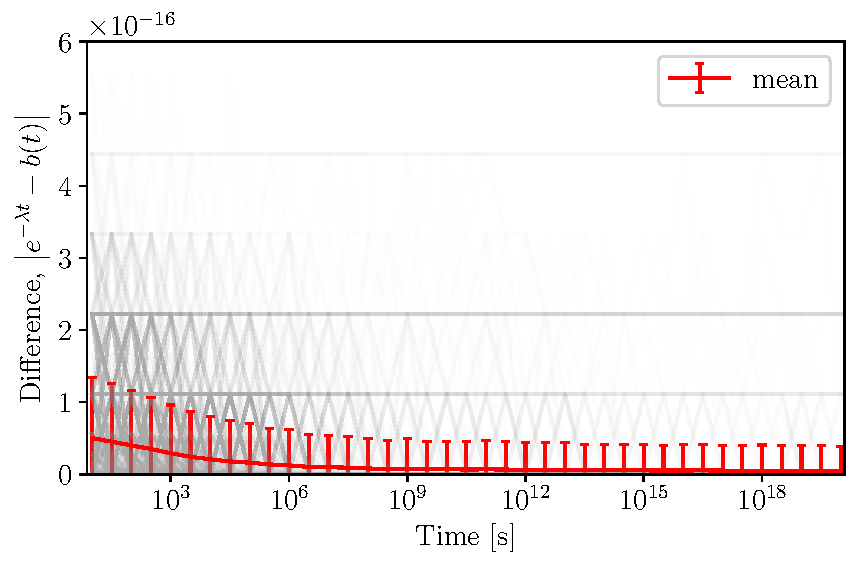
\includegraphics[scale=0.80]{./n1-diff.pdf}
  \caption{The difference between known decay of initial nuclide and the
           binary bateman solution for all 3491 nuclides. The red line
           is the average of the absolute value of difference with
           error bars repesenting 1 standard deviation. The gray lines
           are curves for a subselection of example nuclides which comprise
           the mean.}
  \label{fig-n1}
\end{figure}

As can be seen from Fig.~\ref{fig-n1}, the mean difference tends to zero for
higher decay times.  Moreover, this mean difference curve itself seems to
follow an exponential decay. Importantly, all values in Fig.~\ref{fig-n1}
fall within what could be resonably expected for floating point error for
\texttt{double} precision computation. Additionally, the gray curves
demonstate that for some indvidual nuclides, the difference has a minimum
modal bound. These can be as high as $2.2\times 10^{-16}$. This higher
difference modes persist at long time scales, even as the mean difference
tends to zero.

\subsection{CRAM Comparison}
\label{subsec-cram}
To verify that the binary formualtion of the Bateman equations as presented in
Eq. (\ref{final-form-a})-(\ref{k-bin-pq-degen-2}) is correct, its implementaion
can be compared to the Chebychev Rational Approximation Method (CRAM)
for transmutation
\cite{pusa2010computing,pusa2012correction}. Recent versions of PyNE (v0.5.4+)
now include a both a binary Bateman solver and a CRAM solver.
The CRAM solver is code generated using SymPy \cite{10.7717/peerj-cs.103},
while the binary Bateman solver is code generated using a custom algorithm.

For the CRAM solver, a decay-only matrix can be constructed from the
fundemental nuclear data. This decay-only matrix, thus, does not include
any transmutation from neutron interactions. This usage is distinct from
most CRAM solves, which are focused on depletion.

To create a fair comparison, both solvers where generated from the same
fundemental set of nuclear data. Half-lives and branch
ratios came from the May 1$^{\mathrm{st}}$, 2017 release of ENSDF
\cite{Bhat1992,ensdfmaintained}. Fission product yeild data was obtained
from published WIMS-D results \cite{aldama2003wims}. Therefore, any differences
in the results between the binary Bateman solver and the CRAM
solver can be ascribed to differences in methodology, not differences in data.

However, it should be noted that CRAM is an approximation and the Bateman
equations are the analytic solution. Therefore, we should expect differences
between these two methods up to the approximation order of CRAM. In practice,
the CRAM order is chosen to be at the level of floating point arithmetic.
Since we generally are dealing with \texttt{double} data (64-bit), rather than
\texttt{float} data (32-bit), the floating point error is expected to be
approximately $10^{-16}$ for an inital unit atom density $N_1(0) = 1$.
Thus the CRAM approximation order is chosen as 16 in the comparsion here.

\section{CONCLUSIONS}

Present your summary and conclusions here.

\section*{NOMENCLATURE}
\label{sec-nomen}

Variables used throughout this paper have are described in Table \ref{nomenclature}.

\begin{table}[!htb]
\centering
\caption{Symbols, Units, \& Meaning}
\label{nomenclature}
\begin{tabular}{|l|l|l|}
\hline
\textbf{Symbol} & \textbf{Units} & \textbf{Meaning} \\
\hline
$C$                  & unitless  & Length of the decay chain \\
$i$                  & unitless  & Index for \ith species, on range $[1, C]$ \\
$j$                  & unitless  & Index for \jth species, on range $[1, C]$ \\
$p$                  & unitless  & Index for \pth species, which is special \\
$q$                  & unitless  & Index for \qth species, whose half-life is the same as $p$ \\
$t$                  & seconds   & Time \\
$t_{1/2,i}$          & seconds   & Half-life of the \ith species \\
$\lambda_i$          & 1/seconds & Decay constant of \ith species, $\ln(2)/t_{1/2,i}$ \\
$N_i(t)$             & 1/cm$^3$  & Number density of the \ith species at time t \\
$\gamma_{i \to i+1}$ & unitless  & Branch ratio bewteen \ith species and its child \\
$\gamma$             & unitless  & Total branch ratio for a chain \\
$k_i$                & unitless  & Coefficients allowing for sum-of-exponentials \\
$a_i$                & 1/seconds & Negative inverse of half-life, $-1/t_{1/2,i}$ \\
\hline
\end{tabular}
\end{table}

% Bibliography
\setlength{\baselineskip}{12pt}
\bibliographystyle{physor}
\bibliography{physor}

\appendix
\gdef\thesection{APPENDIX \Alph{section}}
\section{Sample Appendix 1}
\label{app:a}
If necessary, include Appendices numbered in upper case alphabetical order. This is \ref{app:a}.

\end{document}
